\slide{Plan}
{
\tableofcontents
}


\section{Text}


\slide{Listing on multiple comulns}
{
\begin{multicols}{2}
Lorem ipsum dolor sit amet, consectetur adipisicing elit, sed do eiusmod tempor incididunt ut labore et dolore magna aliqua. Ut enim ad minim veniam, quis nostrud exercitation ullamco laboris nisi ut aliquip ex ea commodo consequat. Duis aute irure dolor in reprehenderit in voluptate velit esse cillum dolore eu fugiat nulla pariatur. Excepteur sint occaecat cupidatat non proident, sunt in culpa qui officia deserunt mollit anim id est laborum.
\end{multicols}
}


\section{Listings}


\slide{Test module}
{
\begin{itemize}
\item Modules end with "-m"
\item They are self-containing
\end{itemize}
\lstinputlisting{cpp/test-m.hpp}
}


\slide{Test function}
{
\begin{itemize}
\item Functions ends with "-f"
\item Content of file is wrapped into a function call
\end{itemize}
\lstinputlisting{cpp/other-f.hpp}
}


\slide{Multicolumn listing}
{
\tiny{}
\begin{multicols}{2}
\lstinputlisting{cpp/long_source-m.hpp}
\end{multicols}
}


\section{Graphics}


\slide{Full-slide image}
{
\begin{center}
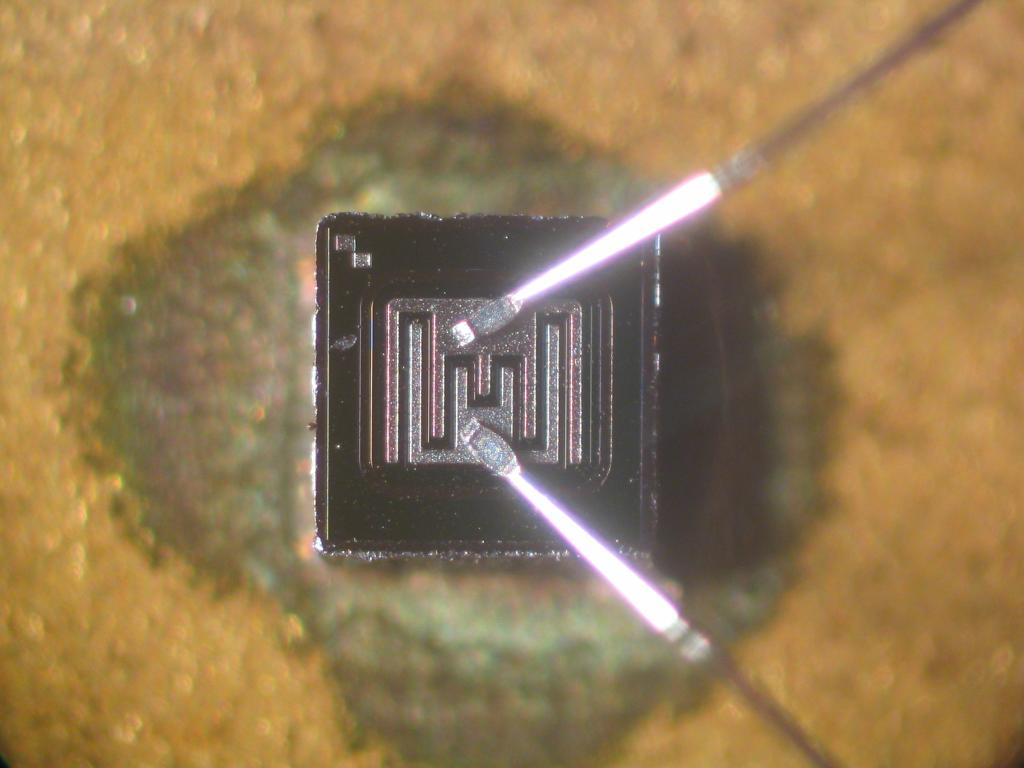
\includegraphics[scale=0.25]{pic/transistor}
\end{center}
}


\slide{Images on different pages}
{
\begin{center}
\includegraphics<1>[scale=0.125]{pic/transistor}
\pause
\includegraphics<2>[scale=0.25]{pic/transistor}
\end{center}
}


\section{Graphviz}


\slide{Hello world}
{
\begin{center}
\includegraphics[scale=0.5]{dot/sample}
\end{center}
}


\section{Gnuplot}


\slide{Function plot}
{
\begin{center}
\includegraphics[scale=0.5]{gnuplot/function}
\end{center}
}


\slide{Discrete plot}
{
\begin{center}
\includegraphics[scale=0.5]{gnuplot/points}
\end{center}
}
